%=================================================================
% CSE 4345 — Big Data Analytics
% Week 1, Part 2: Seminal Research & Case Study
% Department of CSE, Premier University
%
% SEMINAL PAPERS:
%   Laney (2001)  — 3D Data Management: The 3Vs
%   Brewer (2000) — CAP Theorem Conjecture (PODC Keynote)
%   Gilbert & Lynch (2002) — Formal Proof of CAP
%
% CASE STUDY:
%   McKinsey Global Institute (2011) — Big Data: The Next Frontier
%=================================================================

\documentclass[aspectratio=169,10pt]{beamer}

%---------- Packages ----------
\usepackage[utf8]{inputenc}
\usepackage[T1]{fontenc}
\usepackage{booktabs}
\usepackage{xcolor}
\usepackage{tikz}
\usetikzlibrary{shapes.geometric, positioning, arrows.meta, decorations.pathreplacing}
\usepackage{amsmath}
\usepackage{graphicx}
\usepackage{multicol}
\usepackage{enumerate}
\usepackage{array}
\usepackage{textcomp}

%---------- Theme ----------
\usetheme{Madrid}

%---------- Premier University Color Identity ----------
\definecolor{PUNavy}{RGB}{10,36,99}
\definecolor{PUGold}{RGB}{197,151,37}
\definecolor{PULightBlue}{RGB}{210,228,255}
\definecolor{PUTeal}{RGB}{0,100,100}
\definecolor{PUGray}{RGB}{90,90,90}
\definecolor{PURed}{RGB}{160,30,30}
\definecolor{PUGreen}{RGB}{30,120,60}

\setbeamercolor{palette primary}{bg=PUNavy, fg=white}
\setbeamercolor{palette secondary}{bg=PUNavy!85, fg=white}
\setbeamercolor{palette tertiary}{bg=PUNavy!70, fg=white}
\setbeamercolor{palette quaternary}{bg=PUNavy, fg=white}
\setbeamercolor{structure}{fg=PUNavy}
\setbeamercolor{title}{bg=PUNavy, fg=PUGold}
\setbeamercolor{subtitle}{fg=white}
\setbeamercolor{frametitle}{bg=PUNavy, fg=PUGold}
\setbeamercolor{alerted text}{fg=PUGold!85!black}
\setbeamercolor{block title}{bg=PUNavy, fg=white}
\setbeamercolor{block body}{bg=PULightBlue!45}
\setbeamercolor{block title alerted}{bg=PUGold!80!black, fg=white}
\setbeamercolor{block body alerted}{bg=PUGold!12}
\setbeamercolor{block title example}{bg=PUTeal, fg=white}
\setbeamercolor{block body example}{bg=PUTeal!10}
\setbeamercolor{section in toc}{fg=PUNavy}
\setbeamercolor{itemize item}{fg=PUGold!80!black}
\setbeamercolor{itemize subitem}{fg=PUNavy!70}

\setbeamertemplate{navigation symbols}{}
\setbeamertemplate{itemize item}{\scriptsize\raise1.5pt\hbox{\textbullet}}
\setbeamertemplate{itemize subitem}{\scriptsize\raise1pt\hbox{--}}

%---------- Section separator ----------
\AtBeginSection[]{
  \begin{frame}[plain]
    \vfill
    \centering
    \begin{beamercolorbox}[sep=12pt,center,shadow=true,rounded=true]{block title}
      \usebeamerfont{title}\insertsectionhead\par
    \end{beamercolorbox}
    \vfill
  \end{frame}
}

%---------- Helper: citation box ----------
\newenvironment{paperbox}[1]{%
  \setbeamercolor{block title}{bg=PUNavy!90,fg=PUGold}
  \setbeamercolor{block body}{bg=PUNavy!6}
  \begin{block}{#1}}{%
  \end{block}}

%---------- Title metadata ----------
\title[CSE 4345 \textbar{} Week 1, Part 2]{CSE 4345: Big Data Analytics}
\subtitle{Week 1, Part 2 \textemdash\ Seminal Research \& Case Study}
\author[Dept.\ of CSE]{{\sc Rokan Uddin Faruqui} \\ Professor \\ Department of Computer Science \& Engineering\\[4pt]
       \small University of Chittagong, Chittagong}
\institute{}
\date{CSE, PUC, Spring 2026}


%=================================================================
\begin{document}
%=================================================================

%----------------------------------------------------------------
% TITLE SLIDE
%----------------------------------------------------------------
\begin{frame}
  \titlepage
\end{frame}

%----------------------------------------------------------------
% PART 2 OVERVIEW
%----------------------------------------------------------------
\begin{frame}{Part 2 Overview}
  \begin{columns}[T]
    \column{0.47\textwidth}
      \begin{block}{Today's Agenda}
        \tableofcontents
      \end{block}

    \column{0.50\textwidth}
      \begin{exampleblock}{Seminal Papers Covered}
        \begin{enumerate}
          \item Laney, D. (2001). \textit{3D Data Management}. META Group.
          \item Brewer, E. (2000). \textit{Towards Robust Distributed Systems}. PODC.
          \item Gilbert \& Lynch (2002). \textit{Brewer's Conjecture}. ACM SIGACT.
        \end{enumerate}
      \end{exampleblock}
      \vspace{6pt}
      \begin{alertblock}{Case Study}
        Manyika et al.\ (2011). \textit{Big Data: The Next Frontier for Innovation, Competition, and Productivity}. McKinsey Global Institute.
      \end{alertblock}
      \vspace{4pt}
      \begin{block}{CLO Addressed}
        \textbf{CLO1} — Understand big data characteristics\\
        \textbf{PLO(a)}
      \end{block}
  \end{columns}
\end{frame}

%================================================================
\section{Research Paper 1 — Laney (2001): The 3Vs Origin}
%================================================================

\begin{frame}{Research Landscape: Why These Papers?}
  \begin{center}
  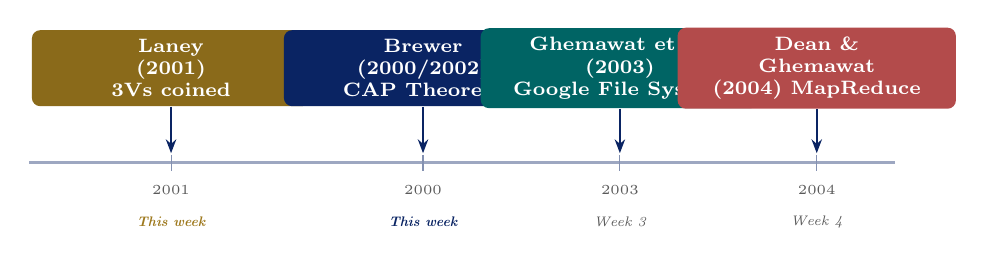
\begin{tikzpicture}[
      node/.style={rectangle, rounded corners=3pt, minimum width=3.5cm,
                   minimum height=0.9cm, text width=3.3cm, align=center,
                   font=\scriptsize\bfseries},
      arr/.style={-{Stealth[length=5pt]}, PUNavy, thick}
    ]
    % Timeline spine
    \draw[PUNavy!40, very thick] (0,0) -- (11,0);

    % Papers
    \node[node, fill=PUGold!70!black, text=white]  (L) at (1.8,1.2)
          {Laney\\(2001)\\3Vs coined};
    \node[node, fill=PUNavy,           text=white]  (B) at (5.0,1.2)
          {Brewer\\(2000/2002)\\CAP Theorem};
    \node[node, fill=PUTeal,           text=white]  (GFS) at (7.5,1.2)
          {Ghemawat et al.\\(2003)\\Google File System};
    \node[node, fill=PURed!80,         text=white]  (MR) at (10.0,1.2)
          {Dean \&\\Ghemawat\\(2004) MapReduce};

    % Year ticks
    \foreach \x/\y in {1.8/2001, 5.0/2000, 7.5/2003, 10.0/2004}{
      \draw[PUNavy!50] (\x,0.1) -- (\x,-0.1);
      \node[font=\tiny, PUGray] at (\x,-0.35) {\y};
    }

    % Arrows from papers to spine
    \draw[arr] (L)   -- (1.8,0.12);
    \draw[arr] (B)   -- (5.0,0.12);
    \draw[arr] (GFS) -- (7.5,0.12);
    \draw[arr] (MR)  -- (10.0,0.12);

    % Week labels
    \node[font=\tiny\itshape, text=PUGold!80!black] at (1.8,-0.75)
          {\textbf{This week}};
    \node[font=\tiny\itshape, text=PUNavy]           at (5.0,-0.75)
          {\textbf{This week}};
    \node[font=\tiny\itshape, text=PUGray]            at (7.5,-0.75)
          {Week 3};
    \node[font=\tiny\itshape, text=PUGray]            at (10.0,-0.75)
          {Week 4};
  \end{tikzpicture}
  \end{center}
  \vspace{6pt}
  \begin{alertblock}{Reading Sequence}
    Laney (2001) defines \emph{what} Big Data is $\;\to\;$ Brewer/Gilbert (2000–2002) defines \emph{why} distributed design is hard $\;\to\;$ GFS (2003) and MapReduce (2004) provide the \emph{engineering solutions}.  This course follows that exact intellectual lineage.
  \end{alertblock}
\end{frame}

%----------------------------------------------------------------
\begin{frame}{Laney (2001): Publication Context}
  \begin{columns}[T]
    \column{0.53\textwidth}
      \begin{paperbox}{Full Citation}
        Laney, D. (2001, February 6). \textbf{3D Data Management: Controlling Data Volume, Velocity and Variety.} META Group Application Delivery Strategies Research Note, File 949.\\[6pt]
        \textbf{Venue:} META Group analyst memo (2 pages)\\
        \textbf{Cited by:} $>$20{,}000 times (Google Scholar, 2024)\\
        \textbf{Impact:} Became the canonical industry and academic definition of Big Data
      \end{paperbox}
      \vspace{6pt}
      \begin{exampleblock}{The Author}
        Doug Laney was a research analyst at META Group (later acquired by Gartner in 2005).  He wrote this as a short practitioner note about \textbf{e-commerce data management challenges}\textemdash not a formal academic paper.
      \end{exampleblock}

    \column{0.44\textwidth}
      \begin{alertblock}{Laney's Own Reflection (2012 Interview)}
        \textit{``It was sort of a throwaway piece.  I had been thinking about the data challenges at e-commerce companies and wrote down three dimensions.  I never expected it to become the definition of an entire era of computing.''}\\
        \hfill\textemdash\,Doug Laney, Gartner Blog, 2012
      \end{alertblock}
      \vspace{6pt}
      \begin{block}{Why Study a 2-page Memo?}
        It illustrates that \textbf{foundational frameworks} need not come from prestigious venues.  The quality of the \emph{insight} matters more than the journal.  This is a recurring theme in Big Data research.
      \end{block}
  \end{columns}
\end{frame}

%----------------------------------------------------------------
\begin{frame}{Laney (2001): The Original 3Vs\textemdash Close Reading}
  \begin{columns}[T]
    \column{0.52\textwidth}
      \begin{paperbox}{Opening Argument (Paraphrased)}
        \textit{``E-commerce has exploded the volume, velocity and variety of information that companies must manage.  Retailers and their trading partners face the challenge of managing large, fast-moving and diverse data from the Web, RFID, point-of-sale sensors and order entry systems.''}
      \end{paperbox}
      \vspace{6pt}
      \textbf{Laney's original definitions:}
      \begin{itemize}
        \item \textbf{Volume:} Transactions at an online retailer generate \textbf{exponentially more} data than equivalent brick-and-mortar operations.  Click-stream data, session logs, product views\textemdash each visit generates thousands of records.
        \item \textbf{Velocity:} The \textbf{time-sensitivity} of data.  Stock prices, fraud signals, and real-time offers must be processed within seconds or the business opportunity is lost.
        \item \textbf{Variety:} Data arriving in \textbf{many formats}\textemdash structured purchase records, semi-structured web logs, unstructured customer reviews.
      \end{itemize}

    \column{0.45\textwidth}
      \begin{alertblock}{The Insight That Made This Seminal}
        Laney was the first to observe that these three dimensions are \textbf{interdependent and compound}:
        \vspace{4pt}
        \begin{itemize}
          \item High velocity $+$ high variety $=$ integration is nearly impossible in real time
          \item High volume $+$ high variety $=$ storage schemas must be flexible
          \item High volume $+$ high velocity $=$ single-node processing cannot keep up
        \end{itemize}
        \vspace{4pt}
        This \textbf{3D problem space} is why no single traditional tool solves Big Data\textemdash you need an \emph{ecosystem}.
      \end{alertblock}
  \end{columns}
\end{frame}

%----------------------------------------------------------------
\begin{frame}{Laney (2001): The E-Commerce Motivation}
  \begin{columns}[T]
    \column{0.52\textwidth}
      \textbf{The year is 2001.  The dot-com boom has just ended.  What data problems were practitioners actually facing?}
      \vspace{8pt}
      \begin{block}{Laney's Observed Challenges}
        \renewcommand{\arraystretch}{1.3}
        \begin{tabular}{p{1.8cm}p{4.2cm}}
          \toprule
          \textbf{Dimension} & \textbf{Observed Problem (2001)} \\
          \midrule
          Volume   & Amazon.com: millions of product pages, billions of click-stream events per month.  No RDBMS could store it all. \\
          Velocity & eBay: real-time auction bids must update in seconds.  Batch-nightly processing was useless. \\
          Variety  & RFID supply-chain data + web logs + customer email = three incompatible formats, no unified query. \\
          \bottomrule
        \end{tabular}
      \end{block}

    \column{0.45\textwidth}
      \begin{exampleblock}{2024 Parallel: Same Problem, 1{,}000$\times$ Scale}
        \begin{itemize}
          \item \textbf{Volume (2024):} Amazon: $>$1.6 million orders per day; petabytes of product images, reviews, fulfillment data
          \item \textbf{Velocity:} Daraz.com.bd: flash-sale order spikes of 10{,}000 orders/minute require real-time inventory sync
          \item \textbf{Variety:} Shopper GPS + purchase history + product image + chatbot transcript + payment gateway log = five different formats in one customer journey
        \end{itemize}
      \end{exampleblock}
      \vspace{4pt}
      \begin{alertblock}{The Enduring Relevance}
        Laney's 3Vs from 2001 describe a problem that has only \textbf{grown more severe}. The framework is still the standard taxonomy in every major cloud provider's documentation (AWS, GCP, Azure) in 2024.
      \end{alertblock}
  \end{columns}
\end{frame}

%----------------------------------------------------------------
\begin{frame}{Laney (2001): Legacy, Extensions, and Critique}
  \begin{columns}[T]
    \column{0.50\textwidth}
      \textbf{What the paper triggered:}
      \begin{itemize}
        \item Gartner adopted 3Vs as official Big Data definition (2012)
        \item IBM extended to \textbf{4Vs} (adding Veracity, 2013)
        \item IDC added \textbf{Value} as the 5th V (2014)
        \item Over 40 papers have proposed additional Vs (Validity, Volatility, Venue, Vocabulary\ldots)
      \end{itemize}
      \vspace{6pt}
      \begin{exampleblock}{The 5Vs Consensus (Gartner / IDC, 2012--2014)}
        \small
        \begin{tabular}{ll}
          \toprule
          V & Added by \\
          \midrule
          Volume, Velocity, Variety & Laney (2001) \\
          Veracity (quality) & IBM (2013) \\
          Value (utility) & IDC (2014) \\
          \bottomrule
        \end{tabular}
      \end{exampleblock}

    \column{0.47\textwidth}
      \begin{alertblock}{Academic Critique of the 3Vs}
        The 3Vs are a \textbf{useful taxonomy}, not a formal theory:
        \vspace{4pt}
        \begin{itemize}
          \item They describe \emph{symptoms}, not solutions
          \item They do not specify \emph{thresholds}: how much volume is ``big''?
          \item They ignore \emph{social and ethical} dimensions of data (privacy, consent, bias)
          \item Kitchin (2014) argues they reinforce a \textbf{techno-deterministic} view that more data always produces better insights
        \end{itemize}
        \vspace{4pt}
        \textbf{Reference:} Kitchin, R. (2014). \textit{The Data Revolution}. Sage. Ch.\,4.
      \end{alertblock}
      \vspace{4pt}
      \begin{block}{Takeaway for Practitioners}
        Use the 3Vs to \textbf{diagnose} problems.  Do not use them to \textbf{justify} adding technology without understanding the specific business value (V5).
      \end{block}
  \end{columns}
\end{frame}

%================================================================
\section{Research Paper 2 — Brewer (2000) \& Gilbert \& Lynch (2002): CAP Theorem}
%================================================================

\begin{frame}{Brewer (2000): The CAP Conjecture}
  \begin{columns}[T]
    \column{0.52\textwidth}
      \begin{paperbox}{Full Citations}
        \textbf{[1]} Brewer, E.\ A.\ (2000). \textbf{Towards Robust Distributed Systems.} Invited Keynote, ACM Symposium on Principles of Distributed Computing (PODC), Portland, Oregon.\\[8pt]
        \textbf{[2]} Gilbert, S.\ \& Lynch, N.\ (2002). \textbf{Brewer's Conjecture and the Feasibility of Consistent, Available, Partition-Tolerant Web Services.} ACM SIGACT News, 33(2), 51--59.
      \end{paperbox}
      \vspace{6pt}
      \begin{block}{About the Authors}
        \textbf{Eric Brewer}: UC Berkeley professor; co-founder of Inktomi (early web search engine), VP of Infrastructure at Google.  His \emph{practitioner} instincts drove the conjecture.\\[4pt]
        \textbf{Seth Gilbert \& Nancy Lynch}: MIT theoreticians who \emph{formally proved} Brewer's conjecture 2 years later.
      \end{block}

    \column{0.45\textwidth}
      \begin{alertblock}{The Conjecture (Brewer, 2000)}
        \textit{``It is impossible for a web service to simultaneously provide all three of the following guarantees:}
        \begin{itemize}
          \item \textit{\textbf{Consistency}: all nodes see the same data at the same time;}
          \item \textit{\textbf{Availability}: a guarantee that every request receives a response;}
          \item \textit{\textbf{Partition tolerance}: the system continues to operate despite arbitrary message loss or failure of part of the system.''}
        \end{itemize}
        \hfill\textemdash\,Brewer, PODC 2000 Keynote
      \end{alertblock}
  \end{columns}
\end{frame}

%----------------------------------------------------------------
\begin{frame}{Gilbert \& Lynch (2002): The Formal Proof}
  \begin{columns}[T]
    \column{0.52\textwidth}
      \begin{block}{Proof Strategy: Contradiction}
        Gilbert \& Lynch used an \textbf{impossibility argument}:
        \vspace{4pt}
        \begin{enumerate}
          \item Assume a system guarantees C, A, and P simultaneously.
          \item Construct a scenario with a network partition: Node 1 and Node 2 cannot communicate.
          \item A write $w$ is sent to Node 1.  A read $r$ is sent to Node 2.
          \item \textbf{Availability} requires Node 2 to respond to $r$.
          \item \textbf{Consistency} requires Node 2's response to reflect $w$.
          \item But \textbf{Partition tolerance} means Node 2 cannot receive $w$ from Node 1.
          \item \textbf{Contradiction} $\Rightarrow$ C, A, P cannot all hold simultaneously. \hfill\textbf{QED}
        \end{enumerate}
      \end{block}

    \column{0.45\textwidth}
      \vspace{4pt}
      \begin{center}
      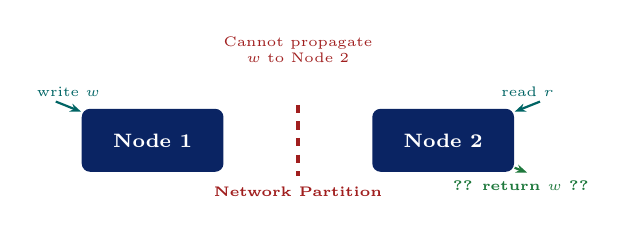
\begin{tikzpicture}[scale=0.82,
          srv/.style={rectangle, rounded corners=3pt, fill=PUNavy, text=white,
                      minimum width=1.8cm, minimum height=0.8cm, font=\scriptsize\bfseries},
          msg/.style={-{Stealth[length=4pt]}, thick}
        ]
        \node[srv] (N1) at (0,0)   {Node 1};
        \node[srv] (N2) at (4.5,0) {Node 2};

        % Client writes
        \draw[msg, PUTeal] (-1.5,0.6) -- node[above,font=\tiny]{write $w$} (N1);
        % Client reads
        \draw[msg, PUTeal] (6.0,0.6) -- node[above,font=\tiny]{read $r$} (N2);

        % Partition
        \draw[PURed, very thick, dashed] (2.25,0.55) -- (2.25,-0.55);
        \node[font=\tiny\bfseries, PURed] at (2.25,-0.8) {Network Partition};

        % Responses
        \draw[msg, PUGreen] (N2) -- node[below,font=\tiny\bfseries]{?? return $w$ ??}(5.8,-0.5);
        \node[font=\tiny, PURed, align=center] at (2.25,1.4)
              {Cannot propagate\\$w$ to Node 2};
      \end{tikzpicture}
      \end{center}
      \vspace{4pt}
      \begin{alertblock}{Design Implication}
        Since partitions \textbf{cannot be prevented} in real networks, every distributed system \emph{must} tolerate P.  The only real design choice is: \textbf{C or A} when a partition occurs.
      \end{alertblock}
  \end{columns}
\end{frame}

%----------------------------------------------------------------
\begin{frame}{CAP Theorem: Real System Choices \& Nuances}
  \begin{columns}[T]
    \column{0.55\textwidth}
      \centering
      \renewcommand{\arraystretch}{1.45}
      \begin{tabular}{p{1.5cm}p{2.8cm}p{2.6cm}}
        \toprule
        \textbf{Choice} & \textbf{Systems} & \textbf{Trade-off} \\
        \midrule
        \textbf{CP} & HBase, ZooKeeper, MongoDB (default) & Returns error instead of stale data during partition \\[4pt]
        \textbf{AP} & Cassandra, DynamoDB, CouchDB & Returns possibly stale data; reconciles later \\[4pt]
        \textbf{CA} & Traditional RDBMS (MySQL, PostgreSQL) & Only works without network partitions (single node) \\
        \bottomrule
      \end{tabular}
      \vspace{8pt}
      \begin{exampleblock}{Bangladesh Example: bKash vs.\ Facebook}
        \small
        \textbf{bKash mobile banking (CP)}: During a network issue, it is better to \emph{reject} a transaction than to process it incorrectly and lose money.\\[4pt]
        \textbf{Facebook timeline (AP)}: During a partition, it is acceptable to show a post from 3 seconds ago rather than blocking the page entirely.
      \end{exampleblock}

    \column{0.42\textwidth}
      \begin{alertblock}{Important Nuance: Kleppmann (2015)}
        \textbf{``Please stop calling databases CP or AP''} --- Martin Kleppmann, \textit{A Critique of the CAP Theorem}, arXiv:1509.05393.
        \vspace{6pt}
        \begin{itemize}
          \small
          \item CAP's definitions are more nuanced than binary classifications suggest
          \item Real systems provide \textbf{tunable consistency} (e.g., Cassandra's consistency levels: ONE, QUORUM, ALL)
          \item \textbf{PACELC model} (Abadi, 2012) extends CAP: even without partitions, there is a Latency vs.\ Consistency trade-off
          \item CAP is a \textbf{useful mental model}, not a precise engineering specification
        \end{itemize}
      \end{alertblock}
  \end{columns}
\end{frame}

%----------------------------------------------------------------
\begin{frame}{Connecting the Papers: From 3Vs to Distributed Design}
  \begin{center}
  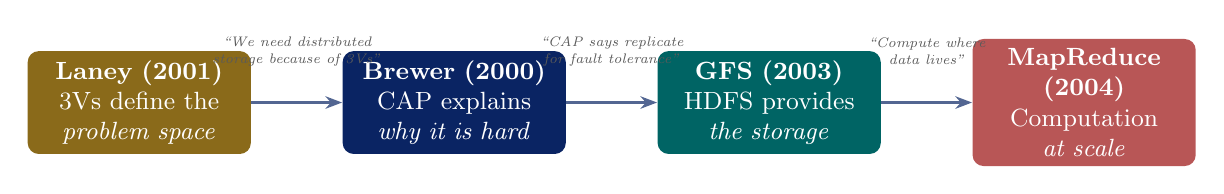
\begin{tikzpicture}[
      box/.style={rectangle, rounded corners=4pt, text width=2.6cm,
                  minimum height=1.1cm, align=center, font=\small},
      arr/.style={-{Stealth[length=6pt]}, PUNavy!70, very thick}
    ]
    \node[box, fill=PUGold!70!black, text=white] (L)
          at (0,0) {\textbf{Laney (2001)}\\\small 3Vs define the\\\small \emph{problem space}};
    \node[box, fill=PUNavy,           text=white] (B)
          at (4,0) {\textbf{Brewer (2000)}\\\small CAP explains\\\small \emph{why it is hard}};
    \node[box, fill=PUTeal,           text=white] (GFS)
          at (8,0) {\textbf{GFS (2003)}\\\small HDFS provides\\\small \emph{the storage}};
    \node[box, fill=PURed!75,         text=white] (MR)
          at (12,0) {\textbf{MapReduce (2004)}\\\small Computation\\\small \emph{at scale}};

    \draw[arr] (L)   -- (B);
    \draw[arr] (B)   -- (GFS);
    \draw[arr] (GFS) -- (MR);

    % Labels on arrows
    \node[font=\tiny\itshape, PUGray, align=center] at (2,0.65)
          {``We need distributed\\storage because of 3Vs''};
    \node[font=\tiny\itshape, PUGray, align=center] at (6,0.65)
          {``CAP says replicate\\for fault tolerance''};
    \node[font=\tiny\itshape, PUGray, align=center] at (10,0.65)
          {``Compute where\\data lives''};
  \end{tikzpicture}
  \end{center}
  \vspace{8pt}
  \begin{alertblock}{The Intellectual Lineage of This Course}
    Laney's 3Vs \textbf{motivated} distributed storage (because a single server cannot handle 3Vs simultaneously) $\to$ Brewer's CAP \textbf{constrained} the design space (you must choose C or A) $\to$ Google's GFS and MapReduce \textbf{implemented} a concrete CP-leaning architecture $\to$ Hadoop \textbf{open-sourced} those ideas.  This entire arc from 2001--2006 forms the foundation of everything you will study in Weeks 2--10.
  \end{alertblock}
\end{frame}

%================================================================
\section{Case Study — McKinsey Global Institute (2011)}
%================================================================

\begin{frame}{About the Report}
  \begin{columns}[T]
    \column{0.52\textwidth}
      \begin{paperbox}{Full Citation}
        Manyika, J., Chui, M., Brown, B., Bughin, J., Dobbs, R., Roxburgh, C., \& Byers, A.H.\ (2011, May). \textbf{Big Data: The Next Frontier for Innovation, Competition, and Productivity.} McKinsey Global Institute.\\[6pt]
        \textbf{Length:} 156 pages\\
        \textbf{Downloaded:} $>$2 million times\\
        \textbf{Cited by:} $>$15{,}000 academic papers\\
        \textbf{Lead author:} James Manyika, Director, McKinsey Global Institute
      \end{paperbox}
      \vspace{6pt}
      \begin{block}{Scope}
        Surveyed Big Data potential across \textbf{five domains}: US healthcare, European public administration, US retail, global manufacturing, and personal location data.  Included interviews with 250 executives across 14 industries.
      \end{block}

    \column{0.45\textwidth}
      \begin{alertblock}{Why It Mattered in 2011}
        This was the first large-scale, cross-industry \textbf{quantified economic analysis} of Big Data's potential value.  Before this report, Big Data was primarily a \emph{technical} term used by engineers.  McKinsey made it a \emph{boardroom} term.
      \end{alertblock}
      \vspace{6pt}
      \begin{exampleblock}{Historical Context (2011)}
        \begin{itemize}
          \small
          \item Hadoop 1.0 had just been released (2011)
          \item Spark did not yet exist (2012)
          \item ``Data Scientist'' was named best job in America by HBR (2012)
          \item AWS was 5 years old; cloud computing was nascent
          \item This report \textbf{triggered the Big Data hiring wave} of 2012--2016
        \end{itemize}
      \end{exampleblock}
  \end{columns}
\end{frame}

%----------------------------------------------------------------
\begin{frame}{Key Quantitative Findings}
  \begin{columns}[T]
    \column{0.55\textwidth}
      \centering
      \renewcommand{\arraystretch}{1.5}
      \begin{tabular}{p{3.6cm}r}
        \toprule
        \textbf{Domain} & \textbf{Estimated Value} \\
        \midrule
        US Healthcare & \alert{\textbf{\$300 billion+/year}} \\
        European Public Sector & \textbf{\texteuro{}100 billion+/year} \\
        US Retail (operating margin) & \textbf{60\%+ increase} \\
        Global Manufacturing & \textbf{\$600 billion+} \\
        Personal location data (EU) & \textbf{\$100 billion+} \\
        \midrule
        \textbf{US talent shortfall (deep analytics)} & \textbf{140{,}000--190{,}000 people by 2018} \\
        \textbf{US manager shortfall (data-savvy)} & \textbf{1.5 million by 2018} \\
        \bottomrule
      \end{tabular}
      \vspace{8pt}
      \begin{block}{Methodology Note}
        Values estimated via expert interviews, revenue-impact modelling, and extrapolation from early big data deployments.  \textbf{Not derived from controlled experiments}\textemdash a key limitation noted by critics.
      \end{block}

    \column{0.42\textwidth}
      \begin{alertblock}{The Headline Argument}
        \textit{``Big data will become a key basis of competition, underpinning new waves of productivity growth, innovation, and consumer surplus.  Leaders in every sector will have to grapple with the implications of big data, not just a few data-oriented managers.''}\\
        \hfill\textemdash\,Manyika et al., 2011, p.\ 1
      \end{alertblock}
      \vspace{6pt}
      \begin{exampleblock}{The Talent Gap Was Under-estimated}
        \small The report predicted 140{,}000--190{,}000 deep analytics jobs needed by 2018.  LinkedIn's 2018 Workforce Report found \textbf{250{,}000+ unfilled data science roles} in the US alone\textemdash the actual gap was \emph{larger} than McKinsey forecast.
      \end{exampleblock}
  \end{columns}
\end{frame}

%----------------------------------------------------------------
\begin{frame}{Healthcare: The Flagship Case}
  \begin{columns}[T]
    \column{0.52\textwidth}
      \begin{block}{US Healthcare: \$300B+ Annual Value Potential}
        McKinsey identified five mechanism categories:
        \vspace{4pt}
        \begin{enumerate}
          \item \textbf{Clinical decision support}: Mining EHR data to identify optimal treatments and reduce diagnostic errors. Potential: \$165 billion.
          \item \textbf{R\&D optimisation}: Mining clinical trial data to reduce drug development cost and time.  Potential: \$70 billion.
          \item \textbf{Public health}: Epidemic detection via syndromic surveillance of pharmacy sales and emergency room data.  Potential: \$30 billion.
          \item \textbf{Fraud and waste detection}: Identifying anomalous billing patterns in Medicare/Medicaid claims.  Potential: \$17 billion.
          \item \textbf{Consumer health}: Mining wearable and app data for preventive care.
        \end{enumerate}
      \end{block}

    \column{0.45\textwidth}
      \begin{exampleblock}{2024 Reality Check: What Was Achieved?}
        \small
        \textbf{Largely realised:}
        \begin{itemize}
          \item Google DeepMind's AlphaFold (2020) --- solved protein structure prediction using big data + deep learning
          \item CMS fraud detection using ML saves \$4B/year (2022 GAO report)
          \item COVID-19 genomic surveillance systems (GISAID) directly applied big data to track variants in real time
        \end{itemize}
        \vspace{4pt}
        \textbf{Underachieved:}
        \begin{itemize}
          \item EHR interoperability remains poor (data silos still exist)
          \item \textbf{HIPAA compliance} slows data sharing; predicted gains require data McKinsey assumed would flow freely
        \end{itemize}
      \end{exampleblock}
  \end{columns}
\end{frame}

%----------------------------------------------------------------
\begin{frame}{Critical Analysis: What Did McKinsey Get Right and Wrong?}
  \begin{columns}[T]
    \column{0.48\textwidth}
      \begin{exampleblock}{What McKinsey Got Right \checkmark}
        \begin{itemize}
          \item \textbf{Talent gap}: understated, not overstated
          \item \textbf{Competitive differentiation}: tech companies that used big data (Netflix, Amazon, Google) dominated their industries
          \item \textbf{Healthcare value}: clinical AI has validated many of the predicted gains
          \item \textbf{Retail personalisation}: Amazon's recommendation engine drives $\approx$35\% of revenue\textemdash enabled by big data
          \item \textbf{Urgency}: The hiring and investment wave that followed this report built the infrastructure now used for AI
        \end{itemize}
      \end{exampleblock}

    \column{0.48\textwidth}
      \begin{alertblock}{What McKinsey Missed \texttimes}
        \begin{itemize}
          \item \textbf{Privacy \& regulation}: No mention of GDPR (2018), CCPA, or the political cost of mass data collection (Cambridge Analytica, 2018)
          \item \textbf{Algorithmic bias}: Big data models can \emph{amplify} discrimination (race, gender, credit scoring)
          \item \textbf{Google Flu Trends cautionary tale (2008--2015)}: Hyped as proof of big data power; failed catastrophically due to \textbf{overfitting and Goodhart's Law}
          \item \textbf{Cloud dominance}: Assumed on-premise Hadoop clusters; actual market moved to AWS/GCP/Azure
          \item \textbf{Deep learning}: Report assumed statistical models; neural networks redefined ``analytics''
        \end{itemize}
      \end{alertblock}
  \end{columns}
\end{frame}

%----------------------------------------------------------------
\begin{frame}{Cautionary Interlude: Google Flu Trends (2008--2015)}
  \begin{columns}[T]
    \column{0.52\textwidth}
      \begin{block}{The Claim (Ginsberg et al., 2009, \textit{Nature})}
        \textit{``We can accurately estimate influenza activity in each region of the United States, up to two weeks ahead of traditional CDC reports, simply by tracking the volume of flu-related Google search queries.''}
      \end{block}
      \vspace{6pt}
      \textbf{Initial results}: Predicted flu activity with $r^2 = 0.97$ correlation to CDC data.  Widely cited as proof that big data could replace traditional surveillance.
      \vspace{6pt}
      \begin{alertblock}{What Went Wrong}
        \begin{itemize}
          \item \textbf{Overfitting}: 45 query terms selected post-hoc from 50 million possibilities
          \item \textbf{Goodhart's Law}: When a measure becomes a target, it ceases to be a good measure.  Media coverage of flu \emph{itself} drove search volume.
          \item \textbf{2012--2013}: Model over-predicted flu activity by \textbf{2$\times$}
          \item \textbf{2015}: Project quietly discontinued by Google
        \end{itemize}
      \end{alertblock}

    \column{0.45\textwidth}
      \begin{exampleblock}{Lessons for Big Data Practitioners}
        \begin{enumerate}
          \item \textbf{Correlation $\neq$ causation}: A high $r^2$ on training data does not guarantee real-world validity
          \item \textbf{Feedback loops}: Human behaviour changes when people know they are being measured
          \item \textbf{Ground truth matters}: Big data \textbf{supplements}, it does not replace, rigorous data collection
          \item \textbf{Reproducibility}: Selecting 45 features from 50M candidates without cross-validation is a \textbf{data dredging} error
        \end{enumerate}
        \vspace{4pt}
        \textbf{Reference:} Lazer et al. (2014). \textit{The Parable of Google Flu: Traps in Big Data Analysis.} Science, 343(6176), 1203--1205.
      \end{exampleblock}
  \end{columns}
\end{frame}

%----------------------------------------------------------------
\begin{frame}{Bangladesh \& South Asia Relevance}
  \begin{columns}[T]
    \column{0.52\textwidth}
      \begin{block}{McKinsey's Emerging-Economy Blind Spot}
        The 2011 report focused exclusively on the USA and Europe. But the McKinsey logic applies directly to Bangladesh:
      \end{block}
      \vspace{6pt}
      \renewcommand{\arraystretch}{1.3}
      \begin{tabular}{p{2.2cm}p{4.2cm}}
        \toprule
        \textbf{Sector} & \textbf{Big Data Opportunity} \\
        \midrule
        Mobile finance & bKash: 65M+ accounts, real-time fraud, credit scoring for the unbanked \\
        Garment (RMG) & Supply-chain optimisation, energy prediction in 4{,}000+ factories \\
        Agriculture & Crop yield prediction from satellite data + weather APIs \\
        Public health & Dengue / cholera syndromic surveillance from pharmacy \& hospital data \\
        \bottomrule
      \end{tabular}

    \column{0.45\textwidth}
      \begin{alertblock}{A2i \& ICT Division Initiatives}
        Bangladesh's \textbf{Aspire to Innovate (a2i)} programme is actively building national data infrastructure:
        \vspace{4pt}
        \begin{itemize}
          \item \textbf{National Data Warehouse}: Integrating 49 ministries' databases
          \item \textbf{NID biometric database}: 110 million records used for KYC in banking and telecoms
          \item \textbf{Health Bulletin DHIS2}: District-level health data aggregation
          \item \textbf{Bangladesh Open Data Portal}: data.gov.bd (launched 2021)
        \end{itemize}
        \vspace{4pt}
        \textit{Each of these is a real-world manifestation of the McKinsey public-sector big data thesis.}
      \end{alertblock}
  \end{columns}
\end{frame}

%================================================================
\section{Guided Discussion \& Live Exercise}
%================================================================

\begin{frame}{Class Discussion Questions}
  \begin{exampleblock}{Instructions}
    Discuss in pairs (5 minutes), then share with class.  There are no single correct answers\textemdash\,justify your position with evidence from today's papers.
  \end{exampleblock}
  \vspace{8pt}
  \begin{enumerate}[\textbf{D1.}]
    \item Laney wrote his 3Vs memo in 2001 to describe e-commerce challenges.  Do you think the \textbf{same three dimensions} are still the most important way to characterise Big Data challenges in 2024, or has the field evolved past this framework?  What would you change or add?
  \end{enumerate}
  \vspace{8pt}
  \begin{enumerate}[\textbf{D2.}]
    \item The McKinsey report predicted massive economic value from Big Data, but also \textbf{missed} the privacy, bias, and regulatory implications entirely.  Does this mean we should be \emph{sceptical} of similar economic projections for AI today?  What should analysts include that McKinsey did not?
  \end{enumerate}
  \vspace{8pt}
  \begin{enumerate}[\textbf{D3.}]
    \item The Google Flu Trends failure is often cited as a warning against ``big data hubris.''  Can you identify a current example in Bangladesh where a big data system might \textbf{fail for similar reasons} (feedback loop, overfitting, missing ground truth)?
  \end{enumerate}
\end{frame}

%----------------------------------------------------------------
\begin{frame}{Live Exercise: Apply the Frameworks}
  \begin{block}{Instructions}
    Individual work, 10 minutes.  Submit on paper or LMS.
  \end{block}
  \vspace{6pt}
  \begin{columns}[T]
    \column{0.48\textwidth}
      \begin{exampleblock}{Exercise A: 5Vs Classification (CLO1)}
        For each of the following data assets belonging to a Bangladeshi e-commerce platform, rate each V on a scale of \textbf{Low / Medium / High} and \textbf{justify in one sentence}:
        \vspace{4pt}
        \begin{enumerate}[(1)]
          \item Daily product sales CSV exported from MySQL at midnight
          \item Real-time GPS location of 500 delivery riders
          \item Customer-uploaded product review photos
          \item HL7 medical certificate required for pharmaceutical products
          \item Historical 3-year order archive (cold storage)
        \end{enumerate}
      \end{exampleblock}

    \column{0.48\textwidth}
      \begin{alertblock}{Exercise B: System Design (CAP)}
        You are the CTO of a new Bangladeshi super-app (like bKash + Shohoz + Chaldal combined).  For each sub-system below, state which \textbf{CAP trade-off} (CP or AP) you would choose and why:
        \vspace{4pt}
        \begin{enumerate}[(1)]
          \item \textbf{Mobile wallet balance}: showing current taka balance
          \item \textbf{Product availability}: showing whether an item is in stock
          \item \textbf{Ride fare estimate}: showing the price before the driver accepts
          \item \textbf{Rider GPS map}: showing real-time driver location on map
        \end{enumerate}
        \vspace{4pt}
        \textit{Hint: Think about the consequence of showing \emph{stale} vs.\ \emph{unavailable} in each case.}
      \end{alertblock}
  \end{columns}
\end{frame}

%================================================================
\section*{References}
%================================================================

\begin{frame}{Full References}
  \begin{block}{Seminal Papers}
    \begin{itemize}
      \small
      \item Laney, D. (2001, Feb 6). \textbf{3D Data Management: Controlling Data Volume, Velocity and Variety.} META Group Research Note, File 949.
      \item Brewer, E.\ A. (2000). \textbf{Towards Robust Distributed Systems.} ACM PODC Keynote, Portland, OR.
      \item Gilbert, S. \& Lynch, N. (2002). \textbf{Brewer's Conjecture and the Feasibility of Consistent, Available, Partition-Tolerant Web Services.} \textit{ACM SIGACT News}, 33(2), 51--59.
      \item Kleppmann, M. (2015). \textbf{A Critique of the CAP Theorem.} \textit{arXiv}:1509.05393. \textit{[Recommended reading]}
      \item Abadi, D. (2012). \textbf{Consistency Tradeoffs in Modern Distributed Database System Design: CAP is Only Part of the Story.} \textit{IEEE Computer}, 45(2), 37--42. \textit{[PACELC]}
    \end{itemize}
  \end{block}
  \vspace{4pt}
  \begin{exampleblock}{Case Study \& Critique}
    \begin{itemize}
      \small
      \item Manyika, J. et al. (2011). \textbf{Big Data: The Next Frontier.} McKinsey Global Institute.
      \item Ginsberg, J. et al. (2009). \textbf{Detecting influenza epidemics using search engine query data.} \textit{Nature}, 457, 1012--1014.
      \item Lazer, D. et al. (2014). \textbf{The Parable of Google Flu: Traps in Big Data Analysis.} \textit{Science}, 343(6176), 1203--1205.
      \item Kitchin, R. (2014). \textbf{The Data Revolution.} Sage. Ch.\,4.
    \end{itemize}
  \end{exampleblock}
\end{frame}

%----------------------------------------------------------------
\begin{frame}[c]
  \begin{center}
    {\Large\bfseries End of Week 1}\\[10pt]
    {\large CSE 4345: Big Data Analytics}\\[8pt]
    \textcolor{PUGray}{\rule{7cm}{0.5pt}}\\[10pt]
    \begin{quote}
      \itshape ``The world is one big data problem.''
    \end{quote}
    \hfill\textemdash\,Andrew McAfee, MIT Sloan School
    \vspace{16pt}
    \begin{block}{\centering Next Week: Week 2 (Part 1 \& Part 2)}
      \centering
      Challenges of Big Data: Extraction, Integration \& Heterogeneous Information\\[4pt]
      \small Seminal Paper: Halevy, Rajaraman \& Ordille (2006) $\cdot$ Case Study: Healthcare Interoperability (HL7/FHIR)
    \end{block}
    \vspace{8pt}
    \textbf{Reading before Week 2:} \textbf{[SA]} Ch.\,2 $\cdot$ \textbf{[TE]} Ch.\,3
  \end{center}
\end{frame}

%=================================================================
\end{document}
%=================================================================
